\chapter{The particle in front of a static shield}\label{cha:entanglement-generation}

The generalized setup of the system described in \cref{cha:first-look} with the addition of a conducting Faraday shield is shown in \cref{fig:4:complete-setup}. As before, the particles $A$ and $B$ are delocalized in cat-states with superposition sizes $\Delta x_A$ and $\Delta x_B$ respectively.
\begin{figure}[!htbp]
  \centering
  \def\svgwidth{\textwidth}
  \input{./../figures/problem.pdf_tex}
  \caption{Schematic depiction of a experimental setup for the detection of gravitationally induced entanglement between two particles $A$ and $B$ with radius $R$. They are separated by a distance of $2L + L_A + L_B$ in arbitrary orientations given by the angles $\alpha$ and $\beta$ with small variations $\theta_{A(B)}$. All variations are assumed to be normally distributed around mean zero with standard deviation $\Delta L_{A(B)}$ and $\Delta \theta_{A(B)}$. The particles are delocalized in a cat state with a separation $\Delta x_{A(B)}$ between the states $\ket{\psi_{A(B)}^1}$ and $\ket{\psi_{A(B)}^2}$. A conducting Faraday shield with thickness $d$ is placed in the center between the particles.}
  \label{fig:4:complete-setup}
\end{figure}
The superpositions are extended in arbitrary orientations $\alpha,\beta \in [0,\pi)$ a distance $L$ away from the shield. Most notably, the configuration of $\alpha = \beta = 0$ represents the same \q{parallel orientation} discussed earlier in \cref{cha:first-look}. 
In the following, the case of $\alpha = \beta = \pi/2$ is referred to as the \q{orthogonal orientation}.
If gravity is assumed to be able to mediate entanglement, the above system can generate entanglement between both particles $A$ and $B$ due to their mutual gravitational interaction.
Placing a Faraday shield in the center between the masses should not substantially influence the gravitational entanglement generation.
However, Casimir interactions between the shield and the masses are still present at small separations.
It is straightforward to convince yourself that these interactions can only give rise to local phases for each cat-state, dependent only on their associated particle-shield separations $L^i_{A(B)}$ ($i = 1,2$).
Such local interactions can - assuming a static shield e.g. at zero temperature - not induce any additional entanglement between the masses.

For a complete picture, one has to consider experimental challenges and limitations in a real experiment. 
Measuring the states after some time to determine their entanglement requires knowledge of the states which can be obtained by e.g. full state tomography.
Some proposals aim to measure a quantity that breaks the CHSH-inequality \cite{Clauser_1969} (i.e. an \q{entanglement wittness}) to proof entanglement that way \cite{Bose_2017,Chevalier_2020}, but the generation of such a witness requires insight into the specifics of the experimental realization.
In this thesis, I will focus on the most general and universally applicable case of measuring the complete density matrix of the system and checking for entanglement using a convenient entanglement measure like the \q{logarithmic negativity} \cite{Plenio_2005} introduced in \cref{sec:2:entanglement-measures}.
The density matrix of a 2 qubit system consists of 16 different entries where only 9 of them are independent \footnote{Using the known characteristics of the density matrix like hermiticity $\rho^\dagger = \rho$ and $\tr \rho = 1$, it is possible to reconstruct $\rho$ from only 9 specific entries.}.
For a full tomography, a lot of measurements of the system have to be made to determine the state in the required precision.
During these measurements, engineering challenges of recreating the identical initial conditions, i.e. the placement of the particles in each consecutive run have to be considered.
Especially stochastic variations in the initial angle $\theta_{A(B)}$ and the separation distance $L_{A(B)}$ for individual measurements are important to consider. Other fluctuations in preparing the experiment such as the measurement time were already considered previously in Ref. \cite{Nguyen_2020}.
Even if it was somehow possible to place the particle at the \textit{exact} same position each measurement, thermal vibrations of the shield induce small noisy variations in the shield-particle separation over a lot of runs.
The masses might get entangled in each run of the measurement, however the measurements might differ slightly due to the varying initial placements of the particles resulting in a final reconstructed state that looks like a mixed state
\begin{equation}
  \rho = \int\limits_{-\infty}^{\infty} \dd X \frac{1}{\sqrt{2\pi}\Delta X} e^{-X^2/2(\Delta X)^2} \ketbra{\psi_X} .
\end{equation}
Here, $\ket{\psi_X}$ is the pure state of a single measurement dependent on the random variable $X = \{\theta_{A(B)}, L_{A(B)}\}$ corresponding to placement inaccuracies between multiple measurements.
These variations are assumed to be normally distributed with mean $\mean{X} = 0$ and standard deviation $\Delta X$ on the basis of the central limit theorem \cite[p. 1195]{Riley_2018}.
In some cases, as for example if the plate is not placed exactly in the center or at a tilt, the variations $\theta_{A(B)}$ and $L_{A(B)}$ are correlated as for example $L_A = -L_B$ holds.
In the most general case, all placement variations are assumed to be independent and are drawn from their respective probability distribution.



\subsection*{Convergence for a finite number of measurements}
Experimentally, it would be very interesting to know how fast the averaged density matrix $\bar{\rho}$ after a finite number of $\#$ measurements converges to the idealized asymptotic mean $\mean{\rho}$ given by eq. \eqref{eq:4:average-density}, which is calculated and analyzed in depth in the next two sections.
After $\#$ measurements, the sample average is given by
\begin{equation}
  \bar{\rho} = \frac{1}{\#} \sum_{k=1}^{\#} \rho(X_k)
\end{equation}
where $\rho(X)$ depends on the random variable $X \in \{\theta_{A(B)}, L_{A(B)}\}$ and $X_k$ is the $k$-th sample drawn from the normal distribution $\mathcal{N}(0, (\Delta X)^2)$ \footnote{Here it isn't strictly required that $X_k$ are normally distributed. As long as they are i.i.d. random variables, any distribution is sufficient for the following argumentation \cite[p. 1195]{Riley_2018}.}.
As $\# \rightarrow \infty$, the law of large numbers and in particular the central limit theorem (CLT) ensures that $\bar{\rho} \rightarrow \mean{\rho}$ \cite[p. 1195]{Riley_2018}.
According to the CLT, the sample average $\bar{\rho}(X)$ fluctuates around $\mean{\rho}$ with a standard deviation given by the Berry-Esseen theorem for independent and identically distributed random variables $X_k$ by $\sigma \sim \#^{-1/2}$ \cite{Berry_1941}.
Thus, if the placements of the particles in each measurement are completely independent from each other, the rate of convergence to the ideal mean $\mean{\rho}$ is governed similar to the shot-noise limit by $\mathcal{O}(1/\sqrt{\#})$.

It is however very likely that measurements are mostly performed consecutively in the same trap so that the placements in successive measurements are correlated.
The correlations $\mathrm{Cov}[\rho(X_i), \rho(X_j)] = c_{\abs{i-j}}$ between the $i$-th and $j$-th measurement should therefore decrease with increasing $\abs{i-j}$.
The variance of $\bar{\rho}$ is now dependent of these correlations in the form \cite[p. 1227]{Riley_2018}
\begin{equation}\label{eq:4:correlation-variance}
  \mathrm{Var}[\bar{\rho}] = \frac{1}{\#^2} \sum_{i,j=1}^{\#} \mathrm{Cov}[\rho(X_i), \rho(X_j)] = \frac{1}{\#}\mathrm{Var}[\rho] + \frac{2}{\#^2}\sum_{n=1}^{\# - 1}(\# - n) c_n
\end{equation}
where $\mathrm{Cov}[\rho, \rho] = \mathrm{Var}[\rho]$ was used for the variance of the mean density matrix $\mean{\rho}$.
For correlations $c_n \sim n^{-\alpha}$ ($\alpha < 1$) the sum in eq. \eqref{eq:4:correlation-variance} can by asymptotically calculated by the Euler-Maclaurin formula and scales like
\begin{equation}
  \sum_{n=1}^{\# - 1}(\# - n)n^{-\alpha} \xlongrightarrow{\#\rightarrow\infty} \int_1^{\#}\dd n \, (\#-n)n^{-\alpha} \sim \#^{2-\alpha}
\end{equation}
which results in $\mathrm{Var}[\bar{\rho}] \sim \#^{-\alpha}$. In the asymptotic limit the standard deviation of the sample average $\sqrt{\mathrm{Var}[\bar{\rho}]}$ and thus the convergence rate to the mean $\mean{\rho}$ scales with $\mathcal{O}(1/\sqrt{\#^\alpha})$.
This convergence is arbitrary slow for small $\alpha$ (if the setup does not change a lot between individual measurements) and thus the calculations in the next sections are just a worst-case estimation of the actual experimental results.
If a weaker correlation in the form of $c_n \sim e^{-\alpha n}$ is assumed, the convergence rate is again asymptotically governed by $\mathcal{O}(1/\sqrt{\#})$.



\section{Entanglement generation}\label{sec:4:entanglement-generation}
The averaged state $\mean{\rho}$ after multiple measurements is given by
\begin{equation}\label{eq:4:average-density}
  \mean{\rho} = \int_{-\infty}^{\infty} \dd \theta_A p(\theta_A) \int_{-\infty}^{\infty} \dd \theta_B p(\theta_B) \int_{-\infty}^{\infty} \dd L_A p(L_A) \int_{-\infty}^{\infty} \dd L_B p(L_B) \ \rho(\theta_A, \theta_B, L_A, L_B)
\end{equation} 
where $p(\,\cdot\,)$ represents the Gaussian distributions of the random variables 
$\theta_{A(B)}$ and $L_{A(B)}$ with standard deviations $\Delta \theta$ or $\Delta L$ respectively. 
$\rho(\theta_A, \theta_B, L_A, L_B)$ denotes the state of a single measurement, dependent on the initial setup of the system.
The state $\rho_0$ at $t=0$ is given as before by eq. \eqref{eq:2:initial-state}.
Beyond mutual gravitational interactions, the dynamic phases $\phi^{(i)}_{A(B),\,\mathrm{Cas}}(t)$ are induced on the cat-states $\ket{\psi^{(i)}_{A(B)}}$ ($i = 1, 2$) by Casimir interactions with the Faraday shield.
Using the two different models for the Casimir attraction for large and small separations given by eq. \eqref{eq:3:casimir-sphere-plate-PFA} and eq. \eqref{eq:3:casimir-sphere-plate-PFA}, it follows
\begin{equation}
  \phi^{(i)}_{A(B),\,\mathrm{Cas}}(t) = \frac{t}{\hbar}
  \begin{cases}
     \frac{3 \hbar c}{8 \pi} \left(\frac{\varepsilon_r - 1}{\varepsilon_r + 2}\right) \frac{R^3}{\left(L^{(i)}_{A(B)}\right)^4} & \text{for large separations (LSL)} \\
    \frac{\hbar c \pi^3}{720} \varphi(\varepsilon_r) \left(\frac{\varepsilon_r - 1}{\varepsilon_r + 1}\right) \frac{R}{\left(\mathscr{L}^{(i)}_{A(B)}\right)^2} & \text{for small separations (PFA) .}
  \end{cases}
\end{equation}
Here, $L^{(i)}_{A(B)}$ and $\mathscr{L}^{(i)}_{A(B)} = L^{(i)}_{A(B)}-R$ are the distances between the particles and the shield's surface given by
\begin{align}\label{eq:4:L-casimir}
  L^{(i)}_{A} &= L + L_{A} - \frac{d}{2} \pm_i \frac{\Delta x_{A}}{2} \sin(\alpha + \theta_{A}) \quad \quad \text{and} \\
  L^{(i)}_{B} &= L + L_{B} - \frac{d}{2} \mp_i \frac{\Delta x_{B}}{2} \sin(\beta + \theta_{B})
\end{align}
where $\pm_i = -(-1)^{i}$ distinct between the two cat-states of a single particle.
The gravitationally induced phase between states $\ket{\psi^{(i)}_A}\otimes\ket{\psi^{(j)}_B}$ is given analogue to the previous calculations in \cref{cha:first-look} as
\begin{equation}\label{eq:4:phi-grav}
  \phi^{(ij)}_\mathrm{Grav}(t) = \frac{t}{\hbar} \frac{G M_A M_B}{L^{(ij)}} .
\end{equation}
The separation $L^{(ij)}$ between the particle cat-states $A^{(i)}$ and $B^{(j)}$ is given by
\begin{multline}\label{eq:4:L-gravity}
  L^{(ij)} = \sqrt{\left(2L + L_A + L_B \pm_i \frac{\Delta x_A}{2}\sin(\alpha + \theta_A) \mp_j \frac{\Delta x_B}{2}\sin(\beta + \theta_B)\right)^2 +} \\ \overline{\left(\frac{\Delta x_A}{2}\cos(\alpha + \theta_A) \mp_{i=j} \frac{\Delta x_B}{2}\cos(\beta + \theta_B)\right)^2}
\end{multline}
with $\mp_{i=j} = +(-1)^{\delta_{ij}}$.
Expanding to first order in $\Delta x_{A(B)} \ll L$, $\theta_{A(B)} \ll 1$ and $L_{A(B)} \ll 1$ (which is justified as seen in the following), the averaged evolved state 
$\mean{\rho}$ in eq. \eqref{eq:4:average-density} is analytically obtainable, as shown in \cref{apx:placement-average-density-matrix}.
Assuming $\Delta \theta_A = \Delta \theta_B \equiv \Delta\theta$ and $\Delta L_A = \Delta L_B \equiv \Delta L$, the off-diagonal elements (the so-called \textit{coherences}) decay with
\begin{equation}\label{eq:4:average-density-element}
  \mean{\rho_{kl}} = \frac{1}{4} e^{i \Delta \phi_{kl}(t)} \exp{-\frac{(\xi_{kl})^2}{2} (\Delta\theta)^2 t^2} \exp{-\frac{(\zeta_{kl})^2}{2} (\Delta L)^2 t^2}
\end{equation}
where $\Delta \phi$, $\xi$ and $\zeta$ are substitutes for lengthy expressions given by eq. \eqref{eq:apx:phi-definition}, eq. \eqref{eq:apx:definition-xi} and eq. \eqref{eq:apx:definition-zeta} in the appendix and are dependent on system parameters.
For $\Delta \theta, \Delta L \rightarrow \infty$ or $t\rightarrow \infty$, coherences vanish, resulting in a maximally mixed state with $\tr\rho^2 = 1/4$ - which is not entangled.
For large variations in the initial placement of the particles, one therefore expects the loss of entanglement.

For the special case of two identical particles and $\alpha=\pm\beta$, the logarithmic negativity $E_N$ is approximated to first order as
\begin{equation}\label{eq:4:log-neg-analytical}
  E_N(\mean{\rho}) = \max\left\{ 0,\ \log_2\left(e^{-\gamma}\left(\cosh\gamma + \abs{\sin \phi}\right)\right) \right\}
\end{equation}
where the decoherence parameter $\gamma = \left(\xi^2(\Delta \theta)^2/2 + \zeta^2(\Delta L)^2/2\right)t^2$ is given in eq. \eqref{eq:apx:stochastic-decoherence} and the phase $\phi$ is given by eq. \eqref{eq:4:phi-orientation} in the next section.
Numerical results validate this approximation and are shown in \cref{fig:4:EN-variations} for varying $\Delta \theta$ and $\Delta L$ in the parallel configuration.
\begin{figure}[!htb]
  \centering
  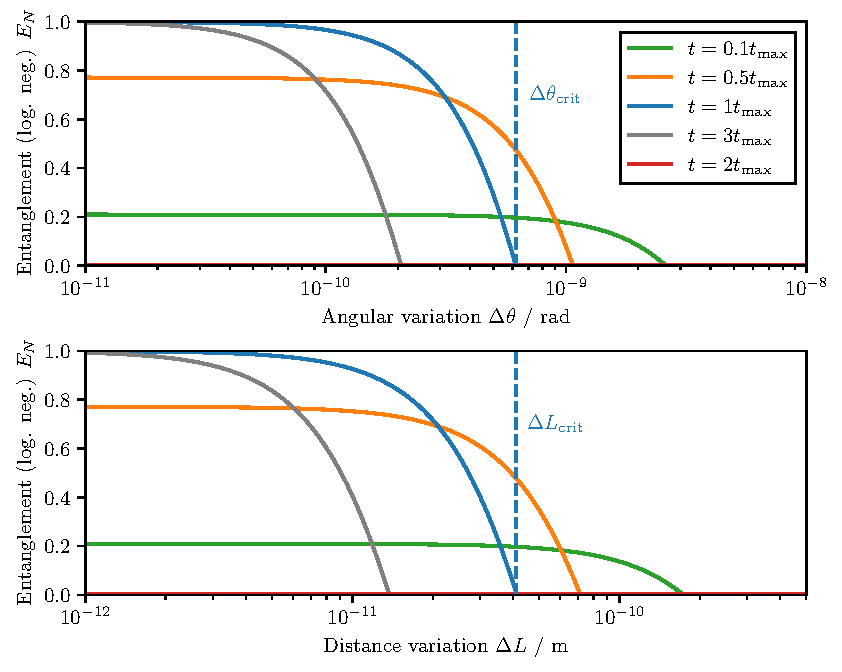
\includegraphics[width=\textwidth]{./../figures/theta-variance/EN-deltaTheta-deltaL.pdf}
  \caption{Entanglement quantified by the logarithmic negativity dependent on the placement variations in the initial setup $\Delta \theta$ and $\Delta L$. The entanglement is shown at different times, where $t_\mathrm{max} \approx 258\si{ms}$ is the time from eq. \eqref{eq:4:t-max}, after which maximal entanglement is reached. At a critical point $\Delta \theta_\mathrm{crit}$ or $\Delta L_\mathrm{crit}$, all entanglement is lost. The used parameters are taken from \cref{tab:paramters}.}
  \label{fig:4:EN-variations}
\end{figure}
For small placement variations, the system remains entangled.
However, once the critical thresholds $\Delta \theta_\mathrm{crit}$ and $\Delta L_\mathrm{crit}$ are surpassed, entanglement is lost entirely.
The critical decoherence threshold $\gamma_\mathrm{crit}$ is given by
\begin{equation}\label{eq:4:critical-point}
  \gamma_\mathrm{crit} = \log(1 + \sqrt{2}) = \mathrm{const.}
\end{equation}
which imposes $\Delta\theta_\mathrm{crit} \propto 1/(\xi t)$ and $\Delta L_\mathrm{crit} \propto 1/(\zeta t)$. 
For the parameters in \cref{tab:paramters}, these thresholds are around $\Delta \theta_\mathrm{crit} \approx 6 \times 10^{-10} \si{rad}$ and $\Delta L_\mathrm{crit} \approx 1.4 \times 10^{-10} \si{m}$, which seems challenging experimentally.
\begin{table}[!t]
  \centering
  \begin{adjustbox}{max width=\textwidth}
    \begin{tabularx}{\textwidth}{c c c c c c c}
      \toprule
      \multirow{2}{*}{Orientation} & \multicolumn{2}{c}{Particle size} & \multirow{2}{*}{$L$} & \multirow{2}{*}{$\Delta x$} & \multicolumn{2}{c}{Shield size $^b$} \\ \cline{2-3} \cline{6-7}
      & Radius $R$ & Mass $M$ $^a$ & & & $d$ & $r_s$\\
      \midrule
      \begin{tabular}{@{}c@{}}Parallel \\ ($\alpha=\beta=0$) \end{tabular} & \begin{tabular}{@{}c@{}}$10\si{\mu m}$ \\ $=10^{-5}\si{m}$\end{tabular} & \begin{tabular}{@{}c@{}}$\approx 10^{-11}\si{kg}$ \\ $=5\times 10^{-4} \, m_p$\end{tabular} & $2R=20\si{\mu m}$ & $100\si{nm}$ & $100\si{nm}$ & $1\si{cm}$ \\
      \bottomrule
      \multicolumn{7}{l}{\footnotesize $^a$ Here $m_p = \sqrt{c\hbar/G}\approx 2.17\times 10^{-8}\si{kg}$ is the Planck mass. $^b$ The required size of the shield is later} \\[-4pt]
      \multicolumn{7}{l}{\footnotesize estimated in section 5.1.} \\[5pt]
    \end{tabularx}
  \end{adjustbox}
  \caption{Default parameters for the setup in \cref{fig:4:complete-setup}. Maximum entanglement is reached after $t_\mathrm{max} = 258\si{ms}$ for these parameters. They were chosen in accordance with multiple proposals \cite{Aspelmeyer_2024,Rijavec_2021}. Both particles are assumed to be identical. The thickness $d$ and radius $r_s$ of the shield is estimated in \cref{sec:5:shield-size}.}
  \label{tab:paramters}
\end{table}
For all these calculations, the radius of the particles is set to $R=10^{-5}\si{m} = 10\si{\mu m}$ with corresponding masses $M=4/3 \pi R^3 \rho_\mathrm{Silica} \approx 1.1\times 10^{-11}\si{kg}$.
A particle-shield separation of $L=2R$ and a superposition size of $\Delta x = 100\si{nm}$ are used.
In the rest of this thesis, if not otherwise specified, these parameters are used as a default.
For convenient retrieval, they are collectively displayed in \cref{tab:paramters}.

These values are consistent with theoretical proposals (see e.g. the Tab. 1 in Ref. \cite{Rijavec_2021}) as they result in a low one-run duration of $t_\mathrm{max}\approx 258\si{ms}$ \cite[Timestamp: 51:00]{Aspelmeyer_2024}, but remain beyond current experimental capabilities.
The largest mass demonstrated in matter-wave interferometry is around $4\times 10^{-23}\si{kg}$ \cite{Fein_2019} with a spatial superposition size of $\Delta x \gtrsim 500\si{nm}$.
In solid-state opto-mechanical systems, quantum control and ground-state cooling have been demonstrated with masses of $10^{-13}\si{kg}$ with mechanical oscillators coupled to superconducting qubits \cite{OConnell_2010}; entangled diamonds with $10^{-11}\si{kg}$ have been observed \cite{Lee_2011} and masses of $10^{-8}\si{kg}$ have been prepared in motional center-of-mass cat-states \cite{Bild_2023}, although with very short coherence times $\lesssim 1\si{\mu s}$.
Also impressive and notable is the cooling of the $\sim 40\si{kg}$ LIGO mirrors to only very few occupied phonon states \cite{Whittle_2021}.
In contrast, the smallest mass with a measurable gravitational force is around $92 \si{mg}$ \cite{Westphal_2021}.
The field of levitated nano-particles has the potential to bridge thw worlds of molecular superposition and mechanical systems, offering exceptional quantum control, high force sensitivity and long coherence times up to seconds \cite{Aspelmeyer_2024}.
Thus many proposals aim to measure quantum entanglement due to gravity between trapped and levitated particles \cite{Krisnanda_2020,GonzalezBallestero_2021}.

Nonetheless, the required accuracy in the placement of the particles appears very challenging experimentally.
However, looking at the entanglement dynamics in \cref{fig:4:EN-dynamics-variations}, for shorter times $t<t_\mathrm{max}$, greater variations in particle placement can be tolerated at the cost of reduced entanglement.
\begin{figure}[!htbp]
  \centering
  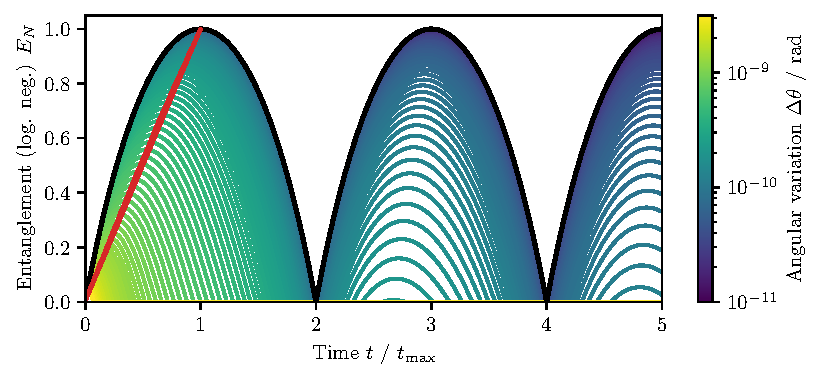
\includegraphics[width=\textwidth]{./../figures/theta-variance/EN-dynamics-delta-theta.pdf}
  \caption{Entanglement dynamics after eq. \eqref{eq:4:log-neg-analytical} for different angular variations $\Delta \theta$ for the parameters used in \cref{tab:paramters}. The black outer most line shows the ideal case without any placement variations and aligns with \cref{fig:2:entanglement-dynamics}. For large variations, entanglement is only observable during a brief window of time with an optimal measurement time colored in red.}
  \label{fig:4:EN-dynamics-variations}
\end{figure}
At these shorter times, the gravitational interaction has not fully entangled the particles, and decoherence (which scales as $\gamma \propto t^2$) has not yet significantly developed.
If achieving full entanglement is not required and \textit{any} amount of entanglement $E_N > 0$ suffices, it may be advantageous to perform measurements at $t < t_\mathrm{max}$.
This, of course, requires ensuring that other entanglement mechanisms contribute smaller entanglement rates (see \cref{cha:the-shield} for further discussion).
Decoherence effects from collisions with air molecules and thermal black-body radiation should also be taken into account.
The optimal measurement time for a required level of entanglement is depicted in \cref{fig:4:time-delta-theta}.
\begin{figure}[!htbp]
  \centering
  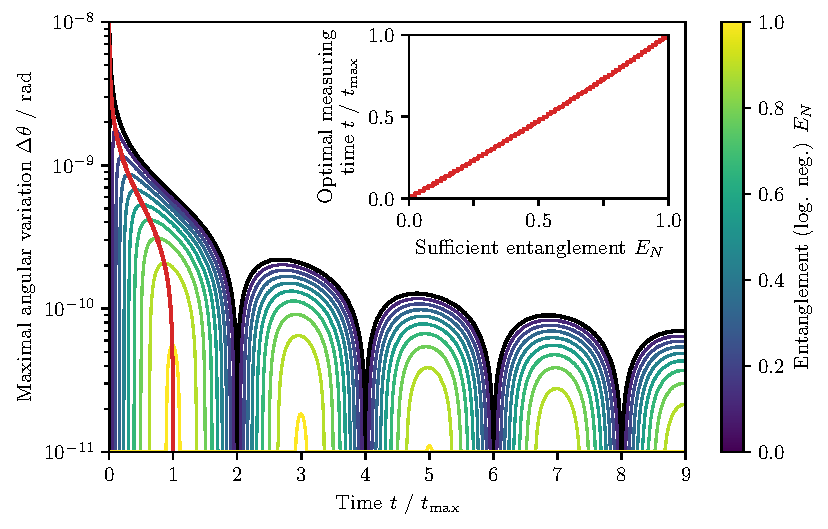
\includegraphics[width=\textwidth]{./../figures/theta-variance/time-delta-theta-crit-EN.pdf}
  \caption{Maximal angular variation for given times after which a specific amount of entanglement $E_N$ is still measurable. The setup parameters are taken from \cref{tab:paramters}. The outer most black line corresponds to the time dependence of $\Delta \theta_\mathrm{crit}$. A fully entangled state with $E_N=1$ is only measurable at $t=t_\mathrm{max}$ with a maximally possible angular variation of around $10^{-11}\si{rad}$. The red curve on the top left shows the optimal measuring time for a specific amount of entanglement and aligns precisely with the red curve in \cref{fig:4:EN-dynamics-variations}. Correspondingly, the red curve in the main figure shows the maximal angular variation for which this goal is reachable. At times $2k t_\mathrm{max},\,k\in\mathbb{N}$ no entanglement can be measured.}
  \label{fig:4:time-delta-theta}
\end{figure}
The figure also provides the corresponding maximum allowable variation for a given time. Conversely, for fixed variations, the optimal measurement time and maximum attainable entanglement can be determined.
It can be seen that at times $2k t_\mathrm{max}, \ k\in\mathbb{N}$ no entanglement is measurable, coinciding with the findings for the ideal scenario in \cref{cha:first-look}. 


\newpage
\section{The optimal setup}\label{sec:4:optimal-setup}
With the general framework in hand, the next logical question to ask is, if the stability against placement-variations can be improved.
The rule of thumb for these optimizations is the following:
Increase the gravitational interaction by either heavier and larger particles or by reducing the separation distance $L$ without substantial sacrifices of experimental realization.
As an example, the stability increases intuitively by increasing the separation distance $L$. However, this does also increase the time $t_\mathrm{max}$ until the maximum amount of entanglement can be measured which would increase the total time  $\sim \# t_\mathrm{max}$ of the experiment with $\#$ individual measurements.
It is not immediately obvious, how the stability and the maximum possible variations $\Delta \theta_\mathrm{crit}$ and $\Delta L_\mathrm{crit}$ behave for the change in parameters.
In the following section, precisely the changing of this stability is discussed for altering the orientation $\alpha, \beta$, the particle-shield separation $L$, the mass $M_A = M_B \equiv M$ and the superposition size $\Delta x_A = \Delta x_B \equiv \Delta x$.

\begin{table}[!h]
  \centering
  \caption{Default parameters for the setup in \cref{fig:4:complete-setup} used in the next sections. The parameters were chosen in accordance with multiple proposals \cite{Aspelmeyer_2024,Rijavec_2021}. Both particles are assumed to be identical with the same mass and superposition size. The thickness $d$ and radius $r_s$ of the shield is estimated in \cref{sec:5:shield-size}.}
  \label{tab:paramters}
  \begin{tabular}{c c c c c c c}
    \toprule
    \multirow{2}{*}{Orientation} & \multicolumn{2}{c}{Particle size} & \multirow{2}{*}{$L$} & \multirow{2}{*}{$\Delta x$} & \multicolumn{2}{c}{Shield size $^b$} \\ \cline{2-3} \cline{6-7}
     & Radius $R$ & Mass $M$ $^a$ & & & $d$ & $r_s$\\
    \midrule
    \begin{tabular}{@{}c@{}}Parallel \\ ($\alpha=\beta=0$) \end{tabular} & \begin{tabular}{@{}c@{}}$10\si{\mu m}$ \\ $=10^{-5}\si{m}$\end{tabular} & \begin{tabular}{@{}c@{}}$\approx 10^{-11}\si{kg}$ \\ $=5\times 10^{-4} \, m_p$\end{tabular} & $2R=20\si{\mu m}$ & $100\si{nm}$ & $100\si{nm}$ & $1\si{cm}$ \\
    \bottomrule
    \multicolumn{7}{l}{\footnotesize $^a$ Here $m_p = \sqrt{c\hbar/G}\approx 2.17\times 10^{-8}\si{kg}$ is the Planck mass. $^b$ The required size of the shield} \\[-4pt]
    \multicolumn{7}{l}{\footnotesize is later estimated in section 5.1.}
  \end{tabular}
\end{table}


\subsection{Orientation}
The arguably easiest parameter to change experimentally is the orientation of the superpositions, which is quantified by $\alpha$ and $\beta$ in \cref{fig:4:complete-setup}.
As already seen in \cref{fig:2:entanglement-dynamics}, the entanglement dynamics are dependent on the orientation.
In the parallel orientation, the states take twice as long as in the orthogonal orientation to become maximally entangled.
In general, it is advantageous to aim for the highest entanglement rate and thus the smallest $t_\mathrm{max}(\alpha, \beta)$, as this requires a shorter coherence time and thus reduces the total time of the experiment.
The previous results from \cref{cha:first-look} can be further generalized for an arbitrary orientation $\alpha, \beta$. The logarithmic negativity is given by
\begin{equation}
  E_N = \log_2\left(1+\abs{\sin\Delta\phi}\right)
\end{equation}
where $\Delta\phi$ is now dependent on the orientation and is defined as (for $\Delta x \ll L$)
\begin{equation}\label{eq:4:delta-phi}
  \Delta \phi = \frac{G M_A M_B t \Delta x_A \Delta x_B}{8\hbar L^3} \left(\sin\alpha\sin\beta-\frac{1}{2}\cos\alpha\cos\beta\right) .
\end{equation}
The maximum entanglement $E_N=1$ is reached for $\Delta\phi = \pm \pi/2$ and thus after a time
\begin{equation}\label{eq:4:t-max}
  t_\mathrm{max}(\alpha,\beta) = \frac{4\pi \hbar L^3}{G M_A M_B \Delta x_A \Delta x_B}\abs{\sin\alpha\sin\beta - \frac{1}{2}\cos\alpha\cos\beta}^{-1}.
\end{equation}
For some specific symmetric cases, the resulting times for different orientations are shown in \cref{fig:4:t-max-orientation}.
\begin{figure}[!htbp]
  \centering
  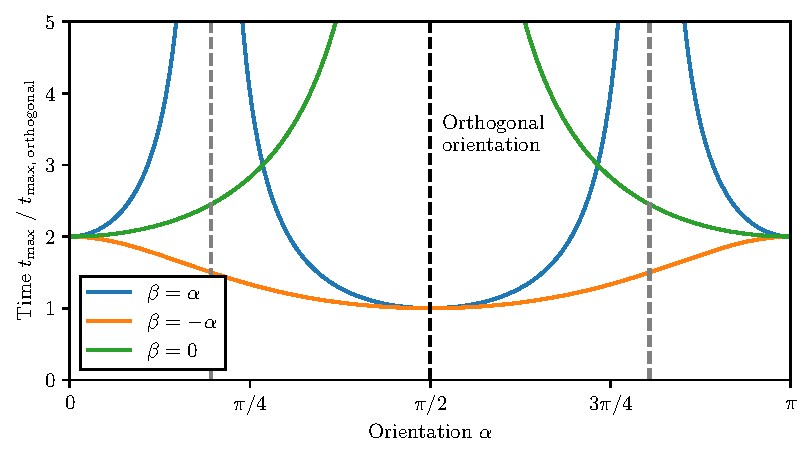
\includegraphics[width=\textwidth]{./../figures/ideal-entanglement/t-max-orientation.pdf}
  \caption{Time $t_\mathrm{max}$ after which maximum entanglement ($E_N = 1$) is reached for different orientations. Only the most interesting and highly symmetric cases $\alpha=\pm\beta$ and $\beta=0$ are shown. The singularity $t_\mathrm{max} \rightarrow \infty$ for $\beta = 0$ and $\alpha = \pi/2$ is expected. The two other singularities at $\alpha = \beta = 2 \arctan(\sqrt{3} \pm \sqrt{2})$ are explainable by the \q{harmonic mean} in \cref{fig:4:harmonic-mean}.}
  \label{fig:4:t-max-orientation}
\end{figure}
The global minima of $t_\mathrm{max}(\alpha,\beta)$ is attained in the orthogonal orientation. This is not surprising considering that this orientation maximizes the \textit{differences in separation distances} between all superposition states.
Much more interesting and surprising are the unanticipated singularities in \cref{fig:4:t-max-orientation} which appear for 
\begin{equation}
  \sin\alpha\sin\beta=\frac{1}{2}\cos\alpha\cos\beta .
\end{equation}
For $\beta=0$ the singularity at $\alpha=\pi/2$ is not surprising. In this configuration, the distances $\ket{\psi^1_A}\leftrightarrow\ket{\psi^{1,2}_B}$ and $\ket{\psi^2_A}\leftrightarrow\ket{\psi^{1,2}_B}$ are identical and thus these states accumulate the same phases, resulting in a factorable global phase.
In the case of $\alpha=\beta$, the two singularities are precisely given in the orientation
\begin{equation}
  \alpha=\beta=2 \arctan(\sqrt{3}\pm\sqrt{2})\approx 90\deg \pm 54.74\deg .
\end{equation}
There does not exist a straight-forward geometric interpretation why no entanglement is generated exactly in this configuration, however all 4 separation distances between the states form the \q{harmonic mean} visualized in \cref{fig:4:harmonic-mean}.
\begin{figure}[!htbp]
  \centering
  \def\svgwidth{\textwidth}
  \input{./../figures/harmonic-mean.pdf_tex}
  \caption{\textbf{left:} The system in the orientation $\alpha=\beta=2\arctan(\sqrt{3}-\sqrt{2})$. For $\Delta x \ll L$, all separation distances exactly form the \textit{harmonic mean}. Here, the phases due to the mutual gravitational interaction precisely cancel out resulting in no entanglement. \textbf{right:} Geometric visualization of the harmonic mean.}
  \label{fig:4:harmonic-mean}
  % COLORFUL:: $\textcolor[HTML]{aa0000}{\blacksquare} = \displaystyle\frac{2}{\frac{1}{\textcolor[HTML]{0044aa}{\blacksquare}}+\frac{1}{\textcolor[HTML]{447821}{\blacksquare}}}$
\end{figure}
Here, in the limit $\Delta x \ll L$ everything local phase precisely cancels out resulting in a loss of entanglement. 
To avoid all these singularities, it is advisable to always take $\alpha=-\beta$, where all orientations result in roughly similar entanglement times $t_\mathrm{max}$, at most only differing by a factor of $2$.

It should come as no surprise that the different orientations exhibit different stabilities. Logically, one would expect the orthogonal configuration to be much more sensitive to angular variations than the parallel one.
In contrary, the parallel configuration should be much more stable against variations in the distance, since no phase difference (\q{dephasing}) is induced between the two superposition states $\ket{\psi^1_{A(B)}}$ and $\ket{\psi^2_{A(B)}}$ of the particle $A$ ($B$).

The effect of different orientations on the stability against angular variations and the behavior of the critical angular variation $\Delta \theta_\mathrm{crit}$ is shown in \cref{fig:4:theta-crit-orientation}.
\begin{figure}[!htbp]
  \centering
  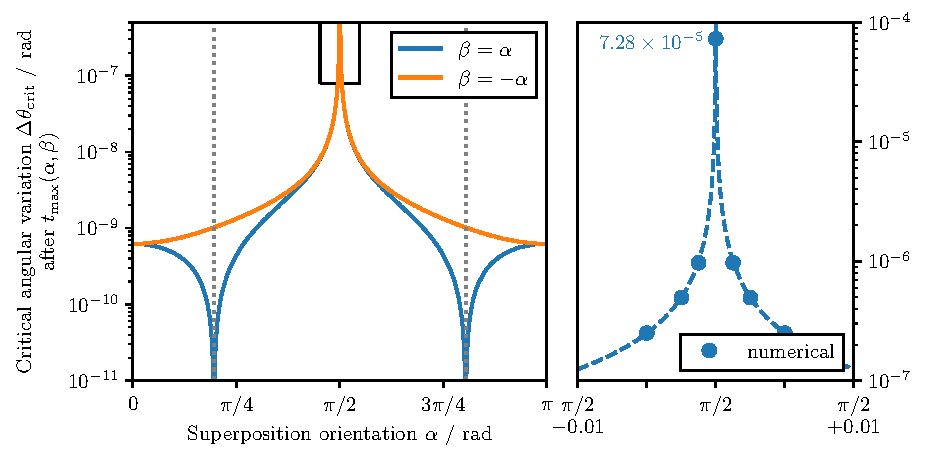
\includegraphics[width=\textwidth]{./../figures/theta-variance/theta-crit-orientation-complete.pdf}
  \caption{Critical angular variation $\Delta \theta_\mathrm{crit}$ for different orientations after the time $t_\mathrm{max}(\alpha, \beta)$ for which maximum entanglement is reached. The \emph{orthogonal orientation} magnified on the right is very stable against angular variations and only numerical methods show a finite stability value. The singularities in the left figure for $\alpha = \beta$ arise from the fact, that these orientations need infinite time to entangle as already seen in \cref{fig:4:t-max-orientation}.}
  \label{fig:4:theta-crit-orientation}
\end{figure}
As expected, the orthogonal configuration is the most stable against these kind of variations. This is, because the dephasing ultimately depends on the distance between the state and the shield $L \pm \Delta x/2 \cos\theta \approx L \pm \Delta x/2 (1 - \theta^2/2)$, which is a only second order effect of the angular variations $\theta$.
This explains the apparent \q{infinitely} good stability in the figure, as the analytical solution only uses first order approximations in $\theta$.
Exact numerical results however cap the stability at $\Delta \theta_\mathrm{crit,\,orthogonal} \approx 7.3\times 10^{-5}\si{rad}$.

Respectively, the stability against distance variations $\Delta L_\mathrm{crit}$ for different orientations is shown in \cref{fig:4:L-crit-orientation}.
\begin{figure}[!htbp]
  \centering
  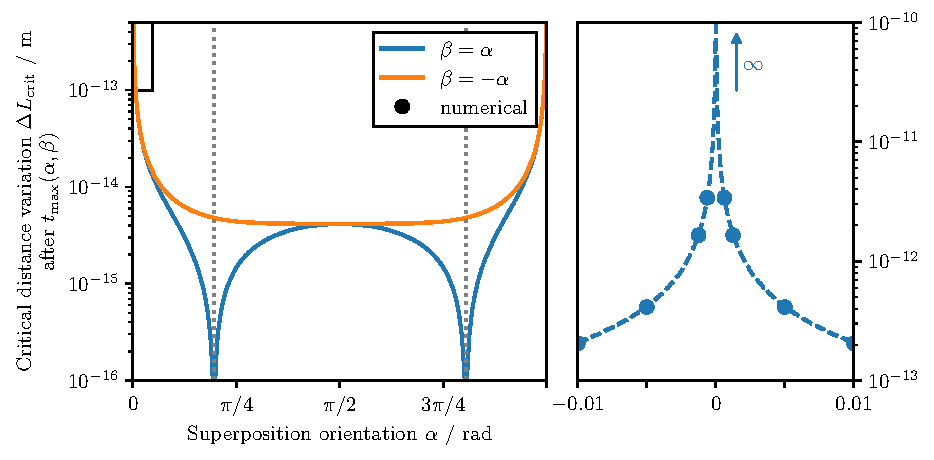
\includegraphics[width=\textwidth]{./../figures/L-variance/L-crit-orientation-complete.pdf}
  \caption{Critical distance variation $\Delta L_\mathrm{crit}$ for different orientations after a time $t_\mathrm{max}(\alpha,\beta)$. Here, the \emph{parallel orientation} (magnified on the left) is infinitely stable against placement variations.}
  \label{fig:4:L-crit-orientation}
\end{figure}
Again aligning with expectations, the parallel configuration is (in theory) exhibits an infinite stability.
One however could argue, that a for this to hold, the uncertainties in the angular placement have to be zero. As could be seen in \cref{fig:4:theta-crit-orientation}, these variations are at most around $\sim 5 \times 10^{-5}\si{rad}$ and thus a realistic upper bound for the minimum required distance variations is given by $\Delta L_\mathrm{crit,parallel} = \Delta L_\mathrm{crit}(\alpha \approx 5\times 10^{-5}\si{rad}) \simeq 4\times 10^{-11}\si{m}$.
It is important to keep in mind, that these stability values can be improved substantially by changing e.g. the separation distance $L$ or the particle size $R$.

Considering these results, the parallel orientation seems to be the only realistic experimental option, even if it requires slightly larger coherence times $t_\mathrm{max}$.
Keeping particle-shield separation variations below $0.01\si{nm}$ - approximately the size of a single atom - is practically impossible,  
especially under the additional consideration of the thermal vibrations of the shield and the particles, which are in the same order of magnitude as seen later in \cref{cha:the-shield}.
With this data on hand, it is possible to generate the stability diagram in \cref{fig:4:optimal-orientation}, showing the optimal orientation in which the most entanglement can be measured.
For most combinations of $\Delta L$ and $\Delta \theta$, entanglement is only given in one certain orientation.
\begin{figure}[!htbp]
  \centering
  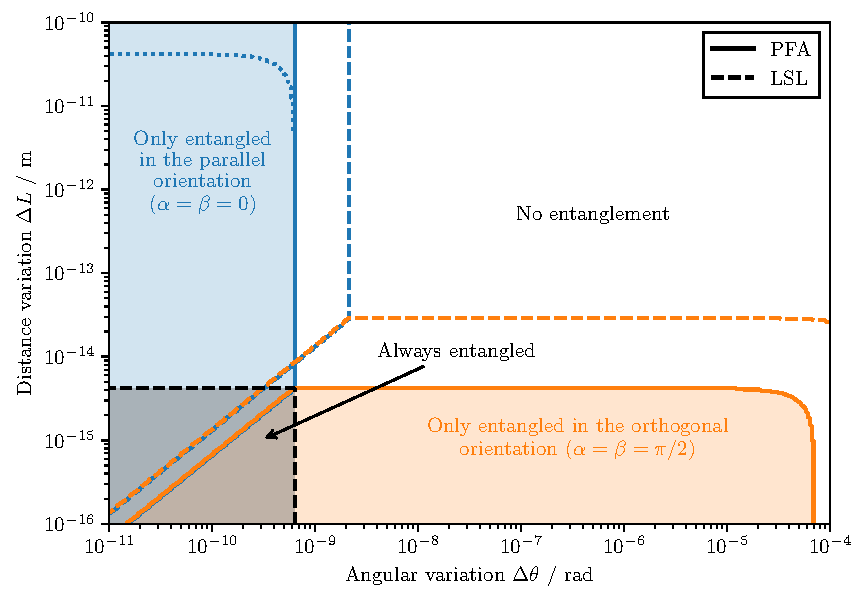
\includegraphics[width=\textwidth]{./../figures/optimize/optimized-orientation-advanced.pdf}
  \caption{Optimal orientation for the experimental setup dependent on the variations in angle $\Delta\theta$ and distance $\Delta L$ for a initial separation distance of $L=2R=2\times 10^{-5}\si{m}$ at time $t_\mathrm{max}$. The different predictions for the proximity-force-approximation (PFA) and the large-separation-limit (LSL) are shown. At a distance of $L=20\si{\mu m}$ the actual casimir interaction is somewhere in the middle between both approximations. In the region where entanglement is given regardless of the orientation (the bottom left), the orientation with \textit{more} entanglement is still colored. The dotted line corresponds to the realistic upper bound discussed in the text.}
  \label{fig:4:optimal-orientation}
\end{figure}


\newpage
\subsection{Separation, mass and superposition size}
It is possible to improve the required stability in placement and consequently the entanglement generation by changing the other parameters shown in \cref{fig:4:complete-setup} besides the orientation. 
It is especially easy to modify the separation distance $L$ during the experiment as one is only limited in the trap stability close to the shield discussed in \cref{sec:4:trapping}. The other parameters like the particle mass $M$ and thus the radius $R$, the particle material and the superposition size $\Delta x$ are considerably more difficult to change.  
One is limited by the experimental implementation of the spatial superpositions. Considering that up to date, the largest spatial superposition of a \q{macroscopic object} is in the order of $\Delta x \sim 500\si{nm}$ for masses of $4\times 10^{-23}\si{kg}$ \cite{Fein_2019}, large changes in the delocalization size $\Delta x$ or the particles mass might be virtually impossible.
However, out of a theoretical standpoint, the effects of all these parameters and the improvements reachable in stability are interesting and considered in the following section.

Beginning with the effect of a larger particle-shield separation $L$, the improvements on angular stability are shown in \cref{fig:4:theta-crit-L}.
\begin{figure}[!htbp]
  \centering
  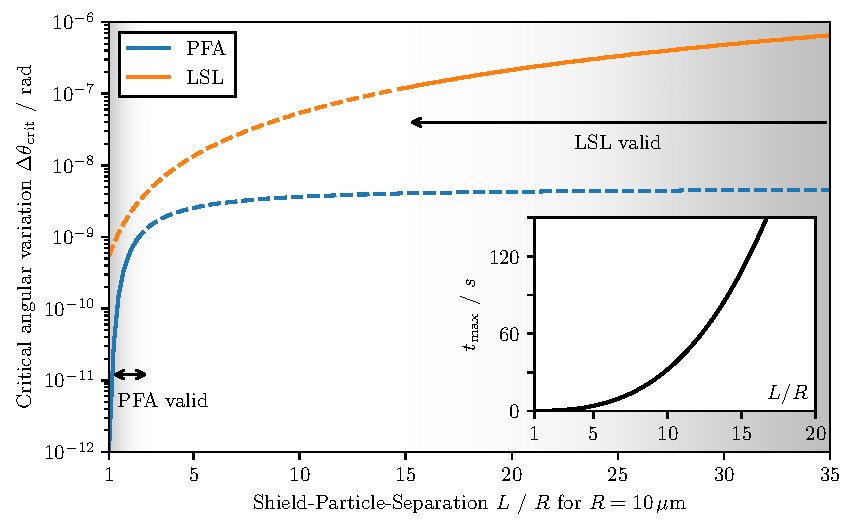
\includegraphics[width=\textwidth]{./../figures/theta-variance/theta-crit-L.pdf}
  \caption{Stability against angular variations for increasing separation distances $L$ in units of $R=10\si{\mu m}$ after a time $t_\mathrm{max}(L)$. The dependence on the radius can be seen in \cref{fig:4:theta-crit-mass}. Two models for the casimir-interaction are shown: The proximity-force-approximation (PFA) and the large-separation-limit (LSL). The regions outside the models validity are indicated with dashed lines. In the bottom right the time $t_\mathrm{max}(L) \propto L^3$ is shown.}
  \label{fig:4:theta-crit-L}
\end{figure}
A similar figure can be created for the stability of distance-variations $\Delta L$, but as already discussed previously, the setup is very (infinitely) stable against small distance variations in the parallel configuration.
It is intuitively clear that a larger separation improves the stability, as the relative effect of the variations $\sim \Delta x \sin\theta \ll L$ decreases and the Casimir potential tends towards zero.
However, a larger separation also increases the time $t_\mathrm{max} \propto L^3$ until the maximum entanglement is built up.
The combination of both effects leads to the result shown in \cref{fig:4:theta-crit-L}.
Due to the strong distance dependence on the casimir model, both limits for either small separations $L \sim R$ (PFA) or large separations $L \gg R$ (LSL) have been compared. 
The \q{real} casimir potential lies somewhere between the two models.
In general, it can be said, that a large separation is desirable, as long as the required coherence times are still reachable.
Looking at the final averaged density matrix $\mean{\rho}$, it is possible to deduce the dependence of $\Delta \theta_\mathrm{crit}$ on the separation $L$. The off-diagonal decoherence terms calculated in \cref{apx:average-density} and given by eq. \eqref{eq:apx:averagted-state-element} scale similar to
\begin{equation}
  \mean{\rho_\mathrm{off-diagonal}} \sim \exp{-\left(\frac{2 \xi_\mathrm{Casimir} \Delta x}{(L - R - d/2)^3} \pm \frac{\zeta_\mathrm{Gravity} \Delta x}{4 L^2} \right)^2 (\Delta \theta)^2 t^2}
\end{equation}
where the second term corresponding to gravitational interactions is much smaller than the first term and thus can be neglected for small $L$.
At the point $\Delta \theta_\mathrm{crit}$ all entanglement is lost leading to $\mean{\rho_{ij}} \rightarrow 0$. Using the analytical results from eq. \eqref{eq:4:theta-crit-analytical} it is possible to get the dependence of $\Delta \theta_\mathrm{crit}$ on $L$ as
\begin{equation}\label{eq:4:delta-theta-scaling-L}
  \Delta \theta_\mathrm{crit} \sim \frac{1}{t_\mathrm{max}} (L - R - d/2)^3 \sim \frac{(L - R - d/2)^3}{L^3} ,
\end{equation}
which aligns very nicely with the blue curve for the PFA in \cref{fig:4:theta-crit-L} ($R^2 = 0.99$ as it is only a approximation). Similar arguments show that for large separations in the LSL the critical angular variation scales with $\Delta \theta_\mathrm{crit} \sim L^2$.

The mass of the particles is determined by their radius $R$ as well as their material.
Most likely, the trapped and levitated particles are made of silica ($\mathrm{SiO_2}$) with a density of $\rho_\mathrm{Silica} = 2648\si{kg/m^3}$, as this material has been used widely in experiments on levitated nanoparticles \cite{Grass_2016,Slezak_2018}. Due to its transparency, silica is very easy to trap in strong optical traps, but even quantum control in magnetic traps has been demonstrated with silica \cite{Slezak_2018}.
For this thesis, I will assume that all trapped particles are made of silica. Otherwise denser or heavier materials like e.g. stable osmium and lead isotopes would be worth considering.
Trapping them in a paramagnetic trap could be theoretically possible and interesting as sufficient masses could already be reached with far fewer atoms and smaller particles, further improving coherence times and quantum control.
The effect on angular stability of a larger and thus heavier particle is shown in \cref{fig:4:theta-crit-mass}.
\begin{figure}[!htbp]
  \centering
  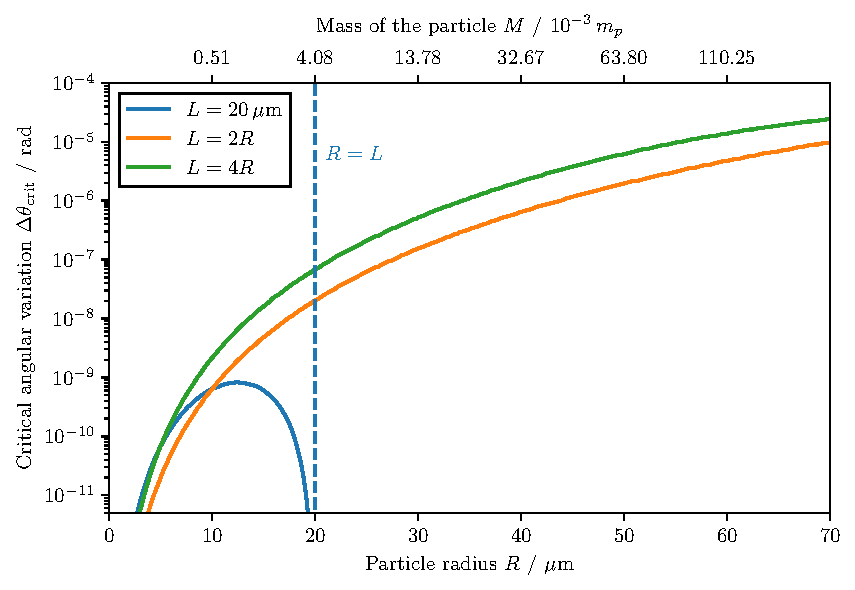
\includegraphics[width=\textwidth]{./../figures/theta-variance/theta-crit-mass.pdf}
  \caption{Critical angular variation $\Delta \theta_\mathrm{crit}$ for different sized particles after a time $t_\mathrm{max}(M)$. The mass of the corresponding particle in units of the Planck mass $m_p = \sqrt{\hbar c / G} \approx 2.176\times 10^{-8}\si{kg}$ is given on the top axis. For particles as large as the separation $R = L$, the surface-to-surface separation is almost zero, resulting in large casimir forces and thus no entanglement.}
  \label{fig:4:theta-crit-mass}
\end{figure}
It is important to note, that the time $t_\mathrm{max}$ scales with $M^{-2}$ and thus effectively with $R^{-6}$, making the effect of a slightly larger sphere very noticeable.
One does need to find the ideal size of the sphere depending on what is possible experimentally: The mass must be large enough for gravity to have a measurable effect but simultaneously small enough for sufficient quantum control in the laboratory. 
Estimations suggest the usage of masses around the order of $10^{-11}\si{kg} \approx 10^{-3}\,m_p$ as being possible \cite{Aspelmeyer_2024}.
The scaling of $\Delta \theta_\mathrm{crit}$ with a changing size $R$ of the particles can be determined similar to before. It turns out, that for a constant separation $L$, the critical angular variation scales with 
\begin{equation}
  \Delta \theta_\mathrm{crit} \sim \frac{(L - R - d/2)^3}{\phi_\mathrm{Casimir}} \frac{1}{t_\mathrm{max}} \sim \frac{(L - R - d/2)^3 R^6}{R}
\end{equation}
whereas for $L \propto R$, the time $t_\mathrm{max} \propto L^3/R^6$ varies additionally resulting in
\begin{equation}
  \Delta \theta_\mathrm{crit} \sim (R - d/2)^3 R^2 .
\end{equation}

The final parameter that theoretically be freely modified, is the size of the superposition $\Delta x$. A larger superposition size would increase the entanglement generation due to gravity because the differences in the distances between all superposition states would increase. Such effects ultimately lead to a faster build-up of entanglement scaling with $t_\mathrm{max} \propto (\Delta x)^{-2}$.
In matter wave experiments, superposition sizes of massive objects up to $\Delta x \approx 500\si{nm}$ were already achieved \cite{Fein_2019}.
These sizes are much smaller than the size of the particle itself at $10\si{\mu m}$.
The effect of the superposition size on stability is shown in \cref{fig:4:theta-crit-superposition-size}.
\begin{figure}[!htbp]
  \centering
  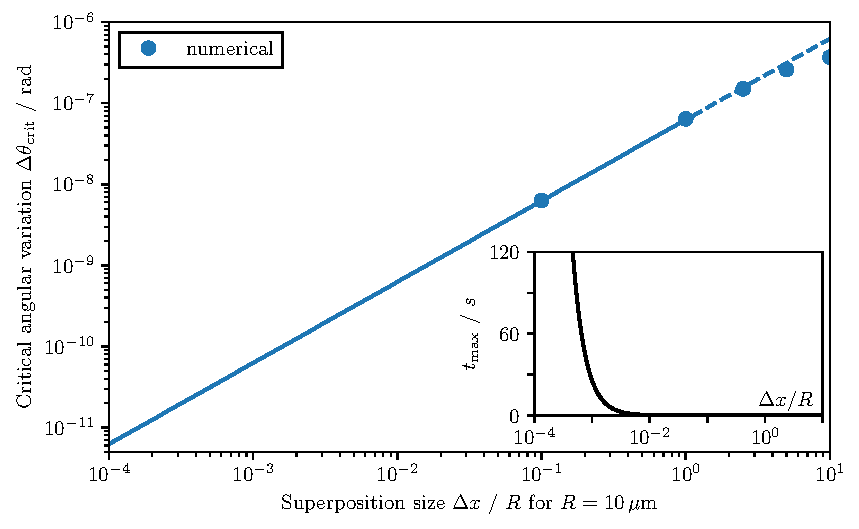
\includegraphics[width=\textwidth]{./../figures/theta-variance/theta-crit-superpos-size.pdf}
  \caption{Effect of the superposition size $\Delta x$ on the critical angular stability $\Delta \theta_\mathrm{crit}$ after a time $t_\mathrm{max}(\Delta x)$. For $\Delta x \gtrsim R$, numerical results are used. In the lower left, the time till maximum entanglement $t_\mathrm{max} \propto (\Delta x)^{-2}$ is shown. For $\Delta x \ll R$, the resulting relation between $\Delta x$ and $\Delta \theta_\mathrm{crit}$ is linear.}
  \label{fig:4:theta-crit-superposition-size}
\end{figure}
For large superposition sizes, the time until maximal entanglement is reached, decreases drastically. In the shorter time, the dephasing due to the casimir effect between the shield and the states is less substantial, increasing the stability against variations in the placement.
A larger superposition size on the other hand results in a greater effect of angular variations $\sim \Delta x \sin(\theta)$.
Both of these effects result in a effective scaling of $\sim \Delta x$, which explains the linear curve\footnote{Here it is shown in a double-logarithmic plot. The relation between $\Delta x$ and $\Delta \theta_\mathrm{crit}$ is nevertheless linear, which can be seen with similar arguments as used previously.}.





\section{Trapping the particle}\label{sec:4:trapping}
The presence of a shield introduces potential challenges to the stability of the particle trap. 
Levitated particles are typically trapped and cooled in ultra-high vacuum using magnetic, optical or electrical radiofrequency Paul traps \cite{GonzalezBallestero_2021}.
These traps differ in the trapping mechanism, but if the particle is cooled close to the ground state, all trapping potentials can be considered \q{harmonic} with trapping frequency $\omega_\mathrm{trap} = 2\pi \times f$.
The strength of the trapping potential $V \propto f^2$ varies across trap types, with frequencies typically ranging from $1\si{Hz}-1\si{kHz}$ for magnetic traps \cite{Slezak_2018} up to $10\si{kHz}-300\si{kHz}$ for optical traps \cite{GonzalezBallestero_2021}. 

If the particle is positioned close to the shield, the Casimir interaction may destabilize the trap or pull the particle onto the shield. The total potential $V_\mathrm{tot}=V_\mathrm{trap} + V_\mathrm{Casimir}$ is shown in \cref{fig:4:trap-eigenstates} for stable and unstable configurations.
\begin{figure}[!htbp]
  \centering
  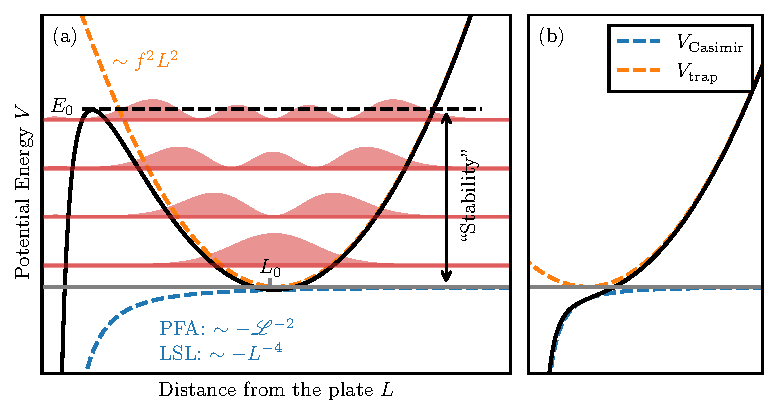
\includegraphics[width=\textwidth]{./../figures/others/trapping-potential-eigenstates.pdf}
  \caption{Visualization of the potential as an overlay of the harmonic trapping potential $V_\mathrm{trap} = m (2\pi f)^2 L^2 / 2$ and the Casimir potential $V_\mathrm{Casimir}$. $f$ is the trapping frequency and $L_0$ the position of the trap. In red, eigenstates of the potential are visualized offset by the eigen-energies.
  \textbf{(a)} Almost harmonic bounded potential which can hold the particle, if its energy is less than $E_0$.
  \textbf{(b)} Potential with no bounded states. Here, trapping is not possible.}
  \label{fig:4:trap-eigenstates}
\end{figure}
The attractive Casimir force $-\nabla V_\mathrm{Casimir}$ displaces the equilibrium trap position closer to the shield by a distance $\Delta x$ given by
\begin{equation}
  \Delta x = \frac{\abs{-\nabla V_\mathrm{Casimir}}}{m (2\pi f)^2} = \frac{2 \hbar c \pi^3}{720} \left(\frac{\varepsilon_r - 1}{\varepsilon_r + 1}\right) \varphi(\varepsilon_r) \frac{R}{\mathscr{L}^3} \frac{1}{m (2\pi f)^2} .
\end{equation}
For $f=1\si{kHz}$ and $L = 2R = 20\si{\mu m}$, this shift is negligibly small, as it is in the order of $\Delta x \approx 10^{-13}\si{m}$.

To determine the stability of a trapped particle with mass $M \propto R^3$ in a trap with frequency $f$ placed at a distance $L_0 > R$ in front of the shield, the number of bound energy-eigenstates in the potential $V_\mathrm{tot}$ is considered.
From \cref{fig:4:trap-eigenstates} it becomes clear, that as long as the particles thermal energy is well below $E_0$, the trap is stable and the particle is bound.
Here, $E_0$ is defined as the local maximum of the potential 
\begin{equation}
  E_0 = \max_{\substack{L\in(R,L_0) \\ \partial_L V(L) = 0}} \left( V_\mathrm{trap} + V_\mathrm{Casimir} \right) .
\end{equation}
If no such local maximum exists, i.e.
\begin{equation}
  \pdv{L} \left( V_\mathrm{trap} + V_\mathrm{Casimir} \right) \neq 0
\end{equation}
for all $L \in (R, L_0)$, the trap is unstable.
Regions of instability are shown in white in the stability diagram \cref{fig:4:trap-stability}.
In the general case, the stability can be measured by computing the number of bound eigenstates $n(E \leq E_0)$ and comparing them with the number of thermally excited states $\bar{n}$.
At a temperature $T$ on average 
\begin{equation}
  \bar{n} = \frac{1}{e^{\beta \hbar \omega} - 1}
\end{equation}
states are occupied, where $\beta = 1/k_B T$ and $\omega = 2\pi f$. This is true, as long as the potential is assumed to be harmonic, which is, as seen shortly, a good approximation.
To find the number of possible bound energy-eigenstates in the potential, the \emph{WKB-approximation} is used.
In this approximation, the energy $E$ of the $n$-th eigenstate of a smooth and appropriately slow varying potential $V(x)$ can be calculated using \cite[p. 163]{Schleich_2001}
\begin{equation}
  \int\limits_{x_1}^{x_2} \dd x \, \sqrt{2m(E-V(x))} = \left(n + \frac{1}{2}\right)\pi\hbar ,
\end{equation}
where $V(x_1) = V(x_2) = E$ are two turning points corresponding to energy $E$.
Conversely, it is possible to use this approximation to numerically estimate the total number of bound states in the potential $V = V_\mathrm{trap} + V_\mathrm{Casimir}$ using
\begin{equation}
  n(E_0) \approx \frac{1}{\hbar \pi} \int_{x_1}^{x_2} \dd x \, \sqrt{2m(E_0 - V(x))},
\end{equation}
which is closely given (highest deviation around $40\%$; averaged relative error $\sim 0.9\%$) by the harmonic approximation $n(E_0) \sim E_0 / \hbar \omega$.
The resulting number of bound states is shown in \cref{fig:4:trap-stability} as well as the stability boundaries at specific temperatures where $\bar{n} = n(E_0)$.
\begin{figure}[!htbp]
  \centering
  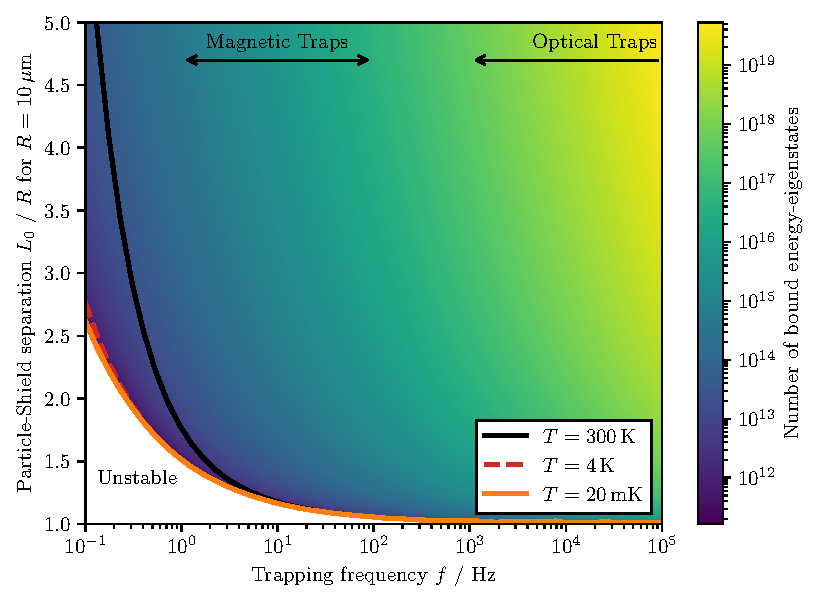
\includegraphics[width=\textwidth]{./../figures/others/trap-stability-with-R.pdf}
  \caption{Stability diagram for different trapping frequencies $f = \omega/2\pi$ and particle-shield separations $L_0$. The number of bound energy-eigenstates for each combination of $f$ and $L_0$ are calculated using the WKB-approximation. The number of thermally occupied states $\bar{n}$ at different Temperatures is overlaid. As an example, for $f=1\si{Hz}$, $\bar{n}(T=300\si{K})\approx 10^{13}$ states are thermally occupied. All regions below these boundaries are unstable. An increase in the radius $R$ and thus the mass $M$ improves the regions of stability massively.}
  \label{fig:4:trap-stability}
\end{figure}
In these calculations, tunneling effects through the potential boundary at $E_0$ are neglected, as they should not influence the results much considering the large number of bound eigenstates.
It turns out, that regardless the type of the trap, a successful trapping even at room temperature should be possible as long as the particle is placed appropriately far away from the trap.
The ability to trap and levitate the masses is therefore not significantly impaired by the presence of the Faraday shield.

\section{Discussions}\label{sec:4:discussion}
The preceding results highlight, that the proposed Faraday shield in experiments on measuring gravitationally induced entanglement entail significant engineering challenges, particularly due to the strict accuracy requirements for particle placement.
Variations must be minimized to a precision of approximately $\Delta L \simeq 10^{-10}\si{m}$ and $\Delta \theta \simeq 10^{-9}\si{rad}$, which are extremely stringent.
Even the rotation of the earth ($\omega_\mathrm{Earth}\approx 7.3\times 10^{-5}\si{rad/s}$) could potentially be problematic, because if small fluctuations in the measurement time $\Delta t \gtrsim 10^{-4}\si{s}$ are present, this corresponds to an additional angular uncertainty of $\omega_\mathrm{Earth}\Delta t \gtrsim \Delta \theta_\mathrm{crit}$.
Adjustments to the experimental parameters in \cref{tab:paramters} have to be made, where especially the separation distance $L$ and the orientation are easily changeable.

The parallel configuration is very stable against variations in the distance and might therefore be favorable (see in \cref{fig:4:optimal-orientation}).
The separation $L$ can be freely chosen and larger distances reduce the effect of placement variations as seen in \cref{fig:4:theta-crit-L}, while simultaneously increasing the required coherence time $t_\mathrm{max} \propto L^3$.

It could also be argued that at a distance of $L \geq 100\si{\mu m} = 10 R$ (compare to \cref{sec:2:experimental-problems}), the Faraday shield would no longer be required because the Casimir forces are approximately ten times weaker than gravitational interactions.
However, the loss of entanglement due to angular and distance variations is not purely due to the Casimir forces between the particle and the shield.
The gravitational coupling also depends on the placement, so that a complete removal of the shield does not fully eliminate the need for high placement accuracy.
Without the shield and by gravitational interaction alone, the critical variations are given by $\Delta \theta_\mathrm{crit,\,ideal} = 1.1 \times 10^{-3}\si{rad}$ and $\Delta L_\mathrm{crit,\,ideal} = 7\times 10^{-4}\si{m}$, which should not pose an engineering problem.

Other parameters, such as particle size and superposition size, may not be easily adjustable without increasing the complexity of quantum control.
Furthermore, particle trapping and levitation is not a limiting factor, as stable trapping is achievable for various configurations (\cref{sec:4:trapping}).

A primary aim of this thesis is to assess whether the Faraday shield allows particles to be brought closer together to enhance gravitational entanglement and reduce coherence times. 
Using the previous results, a optimal experimental parameter space can be determined.
The optimization-goal can be expressed as the following:

One wants to get \textit{as much entanglement as possible} in the \textit{shortest time possible} while allowing for the \textit{largest uncertainties} in the state preparation and considering the limitations in the particles mass as well as in the superposition size.

Without specific constraints, a general optimization is impossible because (if the mass $M$ and the superposition size $\Delta x$ is fixed) coherence time $t \propto L^3$ (eq. \eqref{eq:4:t-max}) and critical angular variation $\Delta \theta_\mathrm{crit} \propto (L-R)^3/L^3$ (for small separations) or $\Delta \theta_\mathrm{crit} \propto L^2$ (for $L \gg R$) cannot be optimized simultaneously.
With constraints such as target coherence time $t_\mathrm{target}$ and/or a minimum placement accuracy, the required sphere-plate separation $L$ as well as maximum measurable entanglement can be determined using the following steps:
\begin{enumerate}
  \item Let us assume that the size of the particle $R$ and consequently the mass $M=4/3 \pi R^3 \rho_\mathrm{Silica}$ as well as the superposition size $\Delta x$ are fixed. An increase in either of them would have a positive effect of the optimization goal stated above, as the time $t_\mathrm{max}$ decreases and the stability against placement variations increases simultaneously.
  \item Given placement accuracies in angular and separation variations determine the optimal orientation $\alpha,\beta$ of the setup as seen in \cref{fig:4:optimal-orientation}. Experimentally reachable coherence times may influence this decision slightly by taking \cref{fig:4:t-max-orientation} into account. Most likely, the most stable orientation is going to be the parallel one with $\alpha = \beta = 0$.
  \item The following ratio given by the entanglement rate eq. \eqref{eq:4:t-max}
  \begin{equation}
    \frac{M^2 (\Delta x)^2}{L^3}t_\mathrm{max} = \frac{4 \pi \hbar}{G}\abs{\sin\alpha\sin\beta-\frac{1}{2}\cos\alpha\cos\beta}^{-1} \sim 10^{-23} \si{kg^2 s/m}
  \end{equation} 
  is fixed therefore \cite{Aspelmeyer_2024}.
  \item In general it is possible to measure at an earlier time $t_\mathrm{target} = \tau t_\mathrm{max}$ (i.e. the coherence time) with $\tau \leq 1$, where less entanglement has been generated but a larger stability against placement variations can be tolerated (see \cref{fig:4:time-delta-theta}). Putting all assumptions together, the product
  \begin{equation}\label{eq:4:fixed-ratio}
    \tau L^3 = \frac{t_\mathrm{target} G M^2 (\Delta x)^2}{8\pi \hbar} = \mathrm{const.}
  \end{equation}
  of measurement time and particle-shield separation is constant.
  \item In the parallel orientation, the distance variations don't matter as the system is very stable against variations in the particle-shield separation. The critical angular variation however scales like $\Delta \theta_\mathrm{crit} \sim (L-R)^3/L^3$ for small distances and like $\Delta \theta_\mathrm{crit} \sim L^2$ at larger distances as shown in \cref{fig:4:theta-crit-L}. It is therefore possible to determine the minimum separation $L_\mathrm{min} > R$ for a given placement accuracy.
  \item Using the required separation, one can calculate $\tau \in (0, 1]$ using eq. \eqref{eq:4:fixed-ratio} and look up the maximal possible entanglement in \cref{fig:4:time-delta-theta} after an evolution time $\tau t_\mathrm{max}$.
\end{enumerate}
As an example, the radius is fixed at $R=10\si{\mu m}$ and the superposition size is $\Delta x = 100\si{nm}$. Let's say that such a particle can be placed with an accuracy of $\Delta \theta = 5 \times 10^{-8} \si{rad}$ and a coherence time of $1\si{s}$ is reachable. 
Using the steps outlined above, the required minimum particle-shield separation is around $L\approx 8R$ and the maximal amount of measurable entanglement is given by $E_N \approx 6.0\times 10^{-2}$.
For more entanglement, either a heavier particle, a larger superposition size, a higher placement accuracy or larger coherence times are required. 
It is therefore possible to bring the particles closer together than without the Faraday shield and still measure entanglement.
One is only limited by the placement accuracy and repeatability.